\chapter*{costruzione dell'immagine}

Le differenze tra computer vision, robot vision e elaborazioni delle immagini 
sono molto sottili:
\begin{itemize}
    \item \textbf{computer vision}: si usano le immagini per comprendere la scena 
    invertendo le proiezioni. In sostanza si parte dall'immagine per ottenere la 
    scena geometrica
    \item \textbf{robot vision}: molto simile a computer vision con la differenza 
    che si utilizzano ulteriori sensori come LIDAR ecc\dots
    \item \textbf{elaborazioni delle immagini}: si occupa di estrarre delle feature 
    dalle immagini date
\end{itemize}

\section{Modelli Pin-Hole}
Le immagini sono la base della computer vision e il modello più semplice di 
proiezione dell'immagine tridimensionale sull'immagine due dimensioni è il pin-hole.

Questo è uno dei primi modelli, nella figura \ref{fig:pin_hole}.
\begin{figure}
    \centering
    \includegraphics*[]{./figure/pin-hole.png}
    \caption{Esempio del modello pin-hole}
    \label{fig:pin_hole}
\end{figure}

Il modello si basa sull'avere una bariera tra il piano due dimensioni e l'oggetto
inquadrato, sul quale è presente un piccolissimo buco, chiamato \textbf{pin-hole},
talmente piccolo da far passare un solo raggio di energia riflessa dall'oggetto e
farlo cadere sul piano di proiezione. Questo modello è una \textbf{proiezione prospettica}
quindi oggetti vicini sono più grandi di oggetti lontani e le rette parallele risultano 
incidenti in un \textbf{punto di fuga}.

A livello puramente geometrico, si ha un piano $uv$ bidimensionale di proiezione (piano immagine)
con centro in $o_i$ (\textbf{punto immagine}), si ha poi il centro dello spazio tridimensionale $xyz$ composto dal 
punto $c$ centrato nel pin-hole (\textbf{pin hole}). L'asse $z$ sarà detto \textbf{asse ottico}, la 
distanza dal punto $c$ e il punto $o_i$ è detta \textbf{lunghezza focale} ed è segnata 
come $f$ (parametro del modello). I punti $P'$, $c$ e $P$ sono punti posizionati sulla stessa retta e questa 
retta viene chiamata, in computer graphics, \textbf{retta di proiezione} di $P$ perché in $P'$ verranno 
proiettati tutti i punti sulla retta. In computer vision non conosciamo $P$ e perciò
si chiamerà \textbf{retta di interpretazione} di $P'$ perché non conosciamo le 
coordinate di $P$ ma solo quelle di $P'$. La formula matematica che descrive questo modello è un sistema di proporzioni:
 
$$P:Z = P':f \equiv \left\{\begin{array}{c}
    \frac{x}{z} = -\frac{u}{f}\\  
    \frac{y}{z} = -\frac{v}{f}\\  
\end{array}\right.$$

\begin{nota}
    Il segno meno nel termine con $f$ perché il piano immagine si trova dietro al 
    centro della proiezione, possiamo pensare nel modello di spostare il piano 
    immagine davanti al centro e questo rimuoverebbe il segno. Nella realtà non 
    è possibile mettere il sensore davati all'obiettivo ma nel modello possiamo 
    farlo per toglierci il meno.
\end{nota}

\begin{figure}
    \centering
    \includegraphics*[scale=0.2]{./figure/pin-hole-modello.jpg}
    \caption{Modello matematico pin-hole}
    \label{fig:pin_hole_model}
\end{figure}

Dove $x,y,z$ sono le coordinate del punto nel mondo, $u,v$ sono le coordinate 
della proiezione e, infine, $f$ è la distanza focale. La formula ha tre diversi 
scopi:
\begin{itemize}
    \item quando fissiamo $x,y,z, f$ abbiamo la proiezione del punto $P$ del mondo 
    sul piano $uv$
    \item quando abbiamo $f,u,v$ allora otteniamo la retta di interpretazione del 
    punto $p'$, perché il sistema è l'intersezione di due piani quindi una retta.
    \item quando conosco $u,v,x,y,z$ effettuamo la calibrazione del modello e otteniamo 
    la distanza focale che ci permette di ottenere quella proiezione
\end{itemize}

Ricorda che quando abbiamo un punto e vogliamo trovare la sua posizione nel mondo
non possiamo ricavare il punto originario della proiezione ma abbiamo solo una retta 
di interpretazione del punto. Questo è dovuto dal fatto che si ottene una retta, 
si può ricavare la distanza originaria usando stereoscopia o sfruttando le informazioni
globali dell'immagine (\textbf{modelbase vision}). 

La \textbf{modelbase vision} è la tecnica per trovare i punti spaziali nel mondo sfruttando la dimensione degli 
oggetti. Tramite il modello Pin Hole possiamo trovare le $x,y$ del punto nello spazio 
ma non possiamo sapere $z$. Per trovarla possiamo sfruttare degli oggetti inquadrati 
di cui è nota la dimensione, ex: targa delle auto.

A livello di modellazione il Pin Hole è perfetto, il problema è che è impossibile 
da realizzare.
Il limite fisico del modello è la dimensione del buco che è impossibile sia 
così piccolo. In aggiunta se fosse così piccolo allora si avrebbe un'immagine molto 
buia, per risolvere questo problema dobbiamo far entrare più luce e questo implica 
il fatto che passano più raggi per ciascun punto che si sovrappongono con i raggi di altri 
punti (\ref{fig:hole}). Alla fine non avremo più i punti immagini, ma bensì avremo 
dei cerchi immagine che si sovrappongono.


\begin{figure}
    \centering
    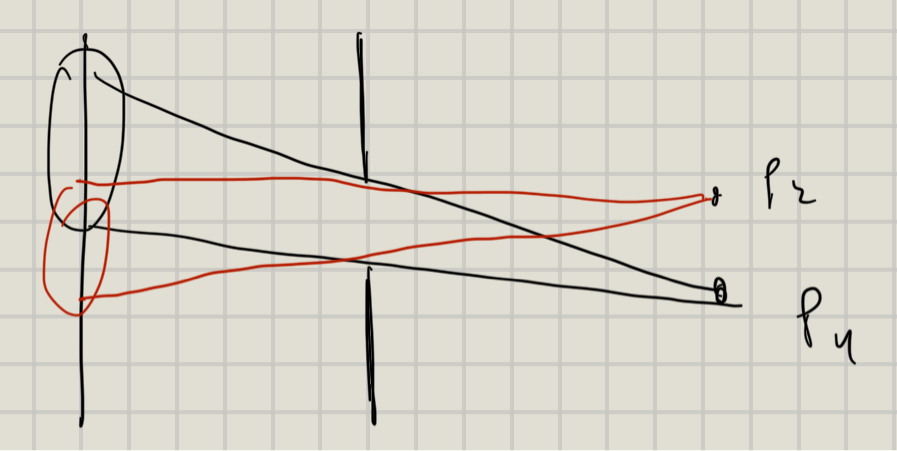
\includegraphics[width=0.5\textwidth]{figure/example_hole.jpg}
    \caption{Esempio di ingrandimento del buco}
    \label{fig:hole}
\end{figure}

Per risolvere questo problema possiamo utilizzare delle lenti fotografiche che 
da un aumento di dimensione del buco concentrano i raggi in un unico punto. Per 
semplicità si consideranno \textbf{lenti sottili}.

\section{Modello di proiezione}
Prima di introdurre le lenti bisogna parlare delle varie proiezioni che si possono 
avere oltre a quella propsettica.

La prima è quella \textbf{ortografica} che è quella utilizzata dai teleobiettivi
delle macchine fotografiche, la proiezione ortografica trasforma tutti i raggi incidenti
sulla lente in raggi paralleli. Per questo si richiede un ristretto angolo focale(\ref{fig:ortography}).

\begin{figure}
    \centering
    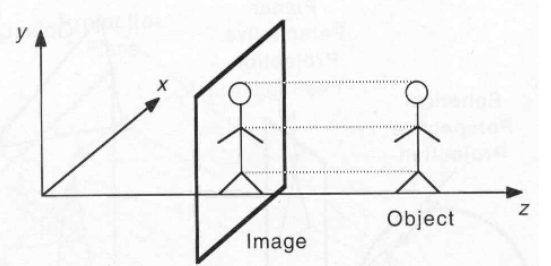
\includegraphics[width=0.5\textwidth]{figure/proiezione_ortografica.png}
    \caption{Esempio di proiezione ortografica}
    \label{fig:ortography}
\end{figure}

La prima è quella \textbf{ortografica scalata} che è quella utilizzata in ambito 
industriale. La proiezione ha una proiezione dei raggi in modo ortografico 
ad una certa distanza per distanze differenti si ha un effetto prospettico. Questo 
è usato nelle industrie per le telecamere che analizzano oggetti alla stessa distanza.
(\ref{fig:scalata_ortography})

\begin{figure}
    \centering
    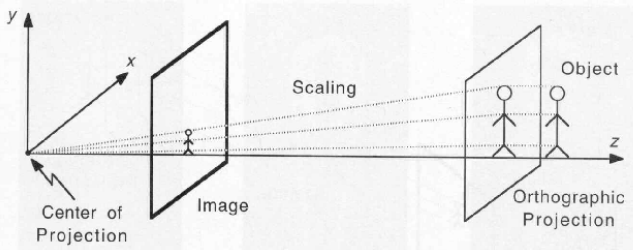
\includegraphics[width=0.5\textwidth]{figure/proiezione_ortografica_scalata.png}
    \caption{Esempio di proiezione ortografica scalata}
    \label{fig:scalata_ortography}
\end{figure}

\section{Lenti sottili}
I dispositivi ottici si possono basare:
\begin{itemize}
    \item riflessione
    \item rifrazione
    \item entrambi
\end{itemize}

Definiremo la \textbf{distanza focale della lente} ovvero la distanza dalla lente 
alla quale si concetrano tutti i raggi paralleli che incidono sulla lente e il 
punto si chiama \textbf{fuoco}. Se arrivano dei raggi che non sono paralleli allora 
il fuoco del punto si sposta dal fuoco della lente in direzione opposta. Nota che 
i raggi se sono paralleli significa che la distanza dalla del punto irradiante è 
infinito, al contrario se non sono paralleli, quindi l'occetto è vicino alla lente 
allora il punto di fuoco non è il fuoco della lente. Quello che regola la focatura 
dei punti è la legge delle \textbf{lenti sottili} 

$$\frac{1}{f} = \frac{1}{z} - \frac{1}{Z}$$

Dove se $f$ è la distanza focale $z$ è la distanza della proiezione dall'altra parte 
della lente e $Z$ è la distanza dell'oggetto dalla lente. Da notare che $z$ e $Z$
sono discordi perché sono posizionati dal lato opposto rispetto alla lente.


La legge si basa sul modello in figura \ref{fig:model_lenses} e il modello si basa 
sullo schema fisico di rifrazione \ref{fig:physical_lenses}.

\begin{figure}
    \centering
    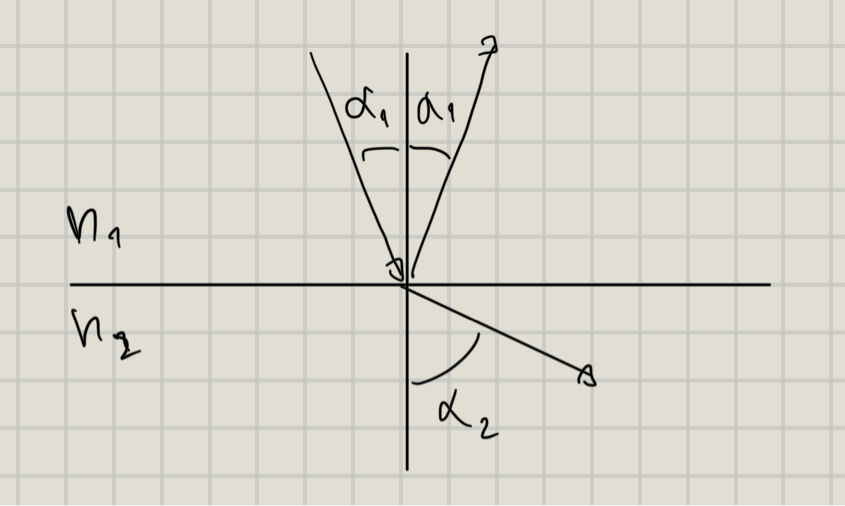
\includegraphics[width=0.5\textwidth]{figure/lenti_fisica.jpg}
    \caption{Schema fisico degli oggetti}
    \label{fig:physical_lenses}
\end{figure}

Dove $\alpha_1$ è l'ancolo di incidenza e riflessione della luce mentre $\alpha_2$
è l'angolo di rifrazione, al tempo stesso $n_1$ e $n_2$ sono i coefficienti di 
riflessione e rifrazione del materiale.

In generale verranno introdotti soltanto lenti basate sulla rifrazione e quindi 
vogliamo minimizzare la riflessione, quindi vogliamo evitare l'\textbf{angolo critico}
 che è l'angolo in cui la luce viene solo riflessa ma non rifratta.

\begin{figure}
    \centering
    \includegraphics*[width=0.5\textwidth]{figure/legge_lente.jpg}
    \caption{Modello della lente}
    \label{fig:model_lenses}
\end{figure}

Da notare che per regolare l'ampienza del buco si parla di regolazione del diaframma,
più è ampio il buco, maggiore è ampio il diaframma e più luce entra. Questo serve 
per regolare l'apertura del diaframma quando la luce è intesa o scarsa. Se è buio 
allora non si vedere nulla.

Per quanto riguarda l'effetto di focatura, un punto è a fuoco quando il diametro di
sfocatura è nullo. Il problema è che quando gli oggetti sono a distanza variabile 
allora dobbiamo trovare il modo di cambiare la sfocatura e questo si basa sullo 
spostare il piano immagine o la lente per raggiungere un diametro nullo. Il problema 
che solo i punti ad una sola distanza sono a fuoco tutti gli altri sono sfocati, 
per risolvere questo problema sfrutta la discretizzazione delle immagini usando i 
pixel. Ovvero quando vogliamo ottenere l'immagine andiamo a ottenere una matrice 
di pixel, questa matrice sarà discreta e si avrà uno spazio tra un pixel e l'altro.
Questo è utile per risolvere il problema della sfocatura infatti per vedere a fuoco 
un punto basta far sì che il diametro di sfocatura non occupi più pixel ma uno solo.
Per regolare il diametro basta agire sul diaframma e sul fuoco, il primo modifica 
l'intervallo di punti a fuoco, mentre il secondo modifica la distanza alla quale questo 
intervallo viene spostato. Esiste una legge che permette di determinare il diametro 
del \textbf{cerchio di sfocamento} e questo è dato da
$$d= \frac{D}{z'}(\overline{z}'-z')$$
Dove $d$ è il diametro del cerchio di sfocatura, $D$ è il diametro del diaframma,
$z'$ è dove va a fuoco il punto scelto e $\overline{z}'$ è dove vanno a fuoco tutti 
i punti a fuoco.

Regolando quidni il diaframma possiamo avere anche profondità di campo diverse della scena
come si può vedere nell'immagine \ref{fig:prof_campo}.

\begin{figure}
    \centering
    \includegraphics*[]{./figure/profondita-campo.png}
    \caption{Esempio profondità di campo}
    \label{fig:prof_campo}
\end{figure}

Delle lenti abbiamo anche l'angolo di visione o \textbf{field of View} che è l'angolo 
di raggi che entrano nell'obiettivo rispetto all'asse ottico. Questo angolo forma 
un cono e successivamente si ha cerchio di riflessione sul sensore o sull'immagine, in generale
si cercherà di avere un cerchio di riflessione più grande rispetto al sensore.

Il FOV può portare a distorsioni dell'immagine per oggetti sul confine dell'occhio visivo:
\begin{itemize}
    \item \textbf{aberrazioni cromatiche}: sbavature di colori dovute alla rifrazione ad 
    angolature diverse dei colori, compare principalmente quando siamo ai confini
    della lente per via delle angolature di rifrazione.
    \item \textbf{distrorsioni}: distorsioni delle proiezioni dei punti, questo è dovuto 
    dalla deviazione dei raggi della lente in angolature diverse. Si possono notare 
    nelle lenti grandangolari. Possiamo avere \textbf{distorsioni radiali} che sono 
    distorsioni dovuti dalla distanza radiale rispetto al centro immagine, se la distorsione
    aumenta quando abbiamo raggi maggiori allora si ha una distorsione a cuscinetto 
    altrimenti a barilotto. In aggiutna abbiamo distorsioni \textbf{tangenziali}
    che sono traslazioni dei punti con un arco predeterminato mantenendo sempre la 
    stessa distanza dal centro immagine, generalmente sono meno intense rispetto 
    a quelle radiali.
\end{itemize}

\begin{nota}
    In coordinate omogenee il modello pin hole è lineare perché quando calcolo 
    la proiezione ottengo un punto 2D in coordinate omogenee allora fino a quando 
    non porto in coordinate normali allora il modello rimane lineare e fino a quando 
    si rimane nello spazio omogeneo allora le distorsioni non vengono incluse.
    Quindi data una foto scattata, devo calcolare la versione non distorta, ottengo 
    l'immagine teorica dopo di che posso trasformare in "3D" usando la matrice inversa 
    delle trasformazioni.
\end{nota}

Un altro effetto sgradevole introdotto dall'ottica è \textbf{vigneting}, è un 
effetto che cresce con la distanza dei punti dal centro immagine. Quando abbiamo 
un'ottica, abbiamo una serie di lenti, quindi quando entrano tutti i raggi si potrebbero 
avere delle rifrazioni non perfette che si scontrano sul cilindro dell'ottica,
provocando l'assorbimento di una parte dell'energia e provocando un'oscurazione del
colore del punto associato a quel punto. Questo può essere un problema quando si 
vuole effettuare delle lavorazioni successive quando si basano sui colori o anche 
sul rilevamento degli edge. Questo si può risolvere cambiando la rappresentazione 
colore.

\begin{nota}
    tutti i problemi delle lenti crescono radialmente.
\end{nota}

\section{Modello realistico}
Il problema del modello Pin Hole è che richiede che il sistema di riferimento del 
mondo sia centrato nel punto di proiezione $c$, che abbia l'asse ottico perfettamente
ortogonale al piano immagine $\pi$ e che passi per il centro immagine. Questo a 
livello ingegneristico è impossibile. Se non ci preoccupiamo di questo allora 
la nostra equazione 
$$\begin{cases}
    u= \frac{fx}{z}\\
    v= \frac{fy}{z}\\
\end{cases}$$
non permetterà di ottenere la posizione reale di un punto quando dall'immagine voglio
ottenere il punto. Non conoscendo con certezza il sistema $xyz$ allora si può 
effettuare una calibrazione. L'idea è di definire un sistema di riferimento mondo 
a piacere e poi definire una rototraslazione per trasferire tutti i punti nello 
spazio camera $xyz$. Per dire la posizione e orientamento di un punto da un sistema di riferimento 
in un altro abbiamo bisogno di un totale di $9$ paramentri ($9$ gradi di libertà)
ovvero, $3$ di posizione di un sistema, $3$ di posizione di un altro sistema 
e $3$ che specificano l'orientamento. I gradi di libertà indipendenti però sono solo 
$6$ perché rappresenteremo solo l'offset come posizione.

Quindi per il modello reale avremo $1$ parametro $f$, $6$ per la POSE, ma in aggiunta
ne abbiamo altri per via della costruzione della camera. Infatti, oltre a questo 
dobbiamo considerare anche il fatto che il sistema $uv$ non è mai centrato nel 
centro immagine ma nella realtà è centrato nell'angolo in alto a sinistra, questo 
richiede di conseguenza di applicare una rototraslazione nel $2D$ omogeneo e quindi 
richiede altri $4$ parametri, $2$ per la posizione e $2$ per la rotazione. Di cui 
indipendenti sono solo $2$ perché in realtà è solo una traslazione. 

In aggiunta, in fase di costruzione non è detto che il sensore che campiona l'immagine 
potrebbe avere degli elementi ricettivi che non sono separati ugualmente, potremmo 
avere problemi legati agli stretching dell'immagine. Questo effetto è chiamato 
\textbf{pixel non quadrato} o \textbf{aspect ratio non unitario} tra i pixel perciò
bisognerà effettuare una trasformazione di scaling. Questo fenomento è descritto 
da un unico parametro.

Un altro problema ingegneristico è sempre dovuta dalla costruzione del sensore, 
infatti si può avere che l'asse $v$ del sistema $uv$ può avere una skew e non essere 
completamente ortogonale con l'asse $u$, questo significa che dobbiamo applicare 
una trasformazione di skew pari alla cotangente dell'angolo di skew (determinato 
da un unico parametro). All'atto pratico 
però questa componente non si conta ma si fissa a $0$, si tiene di default il fatto 
che gli assi sono ortogonali.

In totale i parametri liberi del modello realistico è composto da:
\begin{itemize}
    \item $6$ parametri della rototraslazione dal sistema mondo al sistema camera
    \item $1$ parametro libero per la proiezione dal sistema camera al sistema immagine
    \item $2$ parametri di traslazione del centro immagine
    \item $1$ parametro di scaling del aspect ratio del pixel (evitabile se si ha un 
    rapporto unitario)
    \item $1$ parametro di skew (sempre evitabile perché si considera nullo)
\end{itemize}

\begin{nota}
    Ricorda che spesso si effettua il prodotto tra $f$ e $AR$ e quindi vengono 
    specificati come $f_x,f_y$.
\end{nota}

\begin{definizione}
    Si definiscono \textbf{parametri intrinseci} della camera i parametri della rototraslazione 
    che porta dallo spazio camera allo spazio immagine
\end{definizione}

\begin{definizione}
    Si definiscono \textbf{parametri estrinseci} della camera i parametri della rototraslazione 
    che porta dallo spazio mondo allo spazio camera
\end{definizione}

\section{Calibrazione della proiezione del modello reale}
La \textbf{calibrazione della proiezione} è la fase che determina il tutti i 
parametri del nostro modello reale. Questa è necessaria se vogliamo ottenere fedelmente 
i punti nello spazio.


Per determinare la matrice $M$ di proiezione finale e quindi gli 11 parametri liberi 
abbiamo 2 approcci: DLT e stato dell'arte. Il problema di questi approcci sono 
il fatto che si hanno alcuni punti che hanno \textbf{configurazioni degeneri}. 
La prima configurazione è quando i punti sono \textbf{complanari}. i punti 
devono stare su piani differenti e devono stimolare 
tutti i parametri, se sono complanari effettuiamo una homografia ma non possiamo 
stimare la proiezione prospettica. Inoltre i punti devono essere su piani molto 
diversi altrimenti la matrice diventa malcondizionata.
La seconda configurazione degenere sono punti posizionati su una \textbf{curva cubica} 
che si arrotola su se stessa che 
passa per il centro di proiezione ma questa situazione è difficile da trovare.


\subsection{Regressione lineare}
Ripresa della regressione lineare come modello di stima dei valori.
L'obiettivo del modello di regressione lineare è quello di descrivere la relazione 
tra due variabili attraverso un modello lineare del tipo 
$$\hat{y} = mx + q$$
Date le osservazioni bisogna trovare gli iperparametri $m, q$ con l'obiettivo 
di trovare l'equazione che minimizza $|y - \hat{y}|$. Questo modello può essere utile 
per ridurre il rumore dei punti, ecco questo è lo stesso principio che si effettuerà 
nella direct linear transform. 

\subsection{Direct Linear Transform} 
L'obiettivo sarà quello di ottenere la matrice finale del modello reale $3\times 4$
quindi un totale di $12$ parametri, di cui solo $11$ sono quelli liberi. 

L'operazione di trovare questi parametri è molto complessa, infatti siamo soggetti 
a forti rumori e quindi dovremo sfruttare le stesse metodologie dei modelli di 
regressione. Infatti per la calibrazione non si considera un unico punto, ma bensì
si utilizzano migliaia di punti per ridurre il rumore delle rette di proiezione.
Dobbiamo quindi gestire le incertezze e gli outlier.

Gli 11 parametri liberi del modello si possono considerare come un vettore e questi 
sono in relazione mediante il modello proiettivo. Nota che per effettuare la calibrazione 
noi per ogni punto conosciamo le sue coordinate $uv$ su $\pi$ e le sue coordinate 
$xyz$ nel mondo.

Quindi in sostanza abbiamo per ogni osservazione dei punti reali il vettore composto 
dalla loro posizione del mondo e la loro posizione sullo spazio immagine.
$$\left[\begin{array}{c}
    x\\y\\z\\u\\v
\end{array}\right]$$

Dobbiamo trovare la matrice di trasformazione 
$$M^{3\times 4} = \left[\begin{array}{c}
    \underline{m_1}\\
    \underline{m_2}\\
    \underline{m_3}\\
\end{array}\right]$$

tale che rispetti la seguente relazione 
$$w_1 = \underline{m_1} \cdot \left[\begin{array}{c}
    x\\y\\z\\1
\end{array}\right] \ \ w_2 = \underline{m_2} \cdot \left[\begin{array}{c}
    x\\y\\z\\1
\end{array}\right] \ \ w_3 = \underline{m_3} \cdot \left[\begin{array}{c}
    x\\y\\z\\1
\end{array}\right]$$

Di conseguenza

$$\begin{cases}
    u = \frac{w_1}{w_3}\\
    v = \frac{w_2}{w_3}\\
\end{cases} = \begin{cases}
    u \cdot w_3 - w_1 = 0\\
    v \cdot w_3 - w_2 = 0\\
\end{cases} = \begin{cases}
    u \cdot \underline{m_3} \cdot \left[\begin{array}{c}
        x\\y\\z\\1
    \end{array}\right] - \underline{m_1} \cdot \left[\begin{array}{c}
        x\\y\\z\\1
    \end{array}\right] = 0\\
    v \cdot \underline{m_3} \cdot \left[\begin{array}{c}
        x\\y\\z\\1
    \end{array}\right] - \underline{m_2} \cdot \left[\begin{array}{c}
        x\\y\\z\\1
    \end{array}\right] = 0\\
\end{cases}   $$

quindi data una quintupla di osservazioni posso definire 2 relazioni che vincolano 
la matrice di trasformazione. Per ridurre il rumore della nostra calibrazione si 
utilizzano più osservazioni, proprio nella medesima metodologia della regressione.
Il numero di osservazioni o punti di calibrazione o punti fiduciari sono almeno $6$ perché sono 
11 incognite e 12 equazioni, il problema è che per ridurre il rumore dobbiamo 
aumentare le osservazioni e prendere più punti che non stanno su una sola retta (se ne 
usano un centinaio).

\begin{nota}
    Il ragionamento della proiezione è lo stesso della regressione, per trovare 
    una retta di regressione mi servono almeno $2$ punti secondo gli assiomi geometrici,
    però se vogliamo ridurre il rumore ce ne servono nettamente di più. Nel caso 
    della proiezione diventano almeno $6$ solo che in questo caso il rumore è molto 
    più alto.
\end{nota}

Le osservazioni possono essere prese attraverso l'utilizzo di un piano composto 
da punti neri (punti di cui si prenderanno le osservazioni) su sfondo bianco e le singole coordinate si intercettano in questo modo:
\begin{itemize}
    \item $uv$: si prende l'immagine scattata, si ottengono solo i pixel dei punti 
    si calcola il baricentro di ciascun punto
    \item $xyz$: calcolo la posizione del baricentro dei singoli punti neri nel 
    sistema di riferimento del mondo reale. Ricorda che non ci dobbiamo fermare 
    ad un quantitativo di misure pari al grado di libertà sempre per evitare rumore.
\end{itemize}

Il problema di questo metodo sono \textbf{incertezze} e \textbf{outliers}, perché
essendo un modello regressivo basato sulla differenza dei minimi quadrati allora 
si possono avere questi problemi. 

Questa tecnica è molto onerosa perché richiede le misurazioni nel mondo reale, 
le misurazioni sul piano immagine e ha una ridotta capacità del modello a generalizzare 
fuori dalla nuvola di punti su cui è stata effettuata la calibrazione. Questa 
mancanza di generalizzazione è dovuta dal fatto che si stimano attraverso una regressione 
i parametri della matrice $m_{ij}$ e non si stimano attraverso la struttura degli 
$11$ parametri fisici che porterebbero ad un degradamento ridotta.


\subsection{Stato dell'arte}
La calibrazione allo stato dell'arte si basa sulla:
\begin{itemize}
    \item \textbf{homography}: si utilizza un'omografia tra piani ovvero si hanno 
    una serie di immagini planari che inquadrano oggetti comuni mentre si muove 
    la camera e l'obiettivo e mappare i punti della prima immagine nella seconda.
    \item \textbf{intrinseci/estrinseci}: prima si determinano i parametri intrinseci
    mediante una omografia dei un oggetto planare (scacchiera) e poi si determinano 
    gli estrinseci mediante la stima della posizione degli scacchi.
\end{itemize} 

Questo approccio ci permette di calcolare i parametri di distorsione.